\documentclass[a4paper,twoside,12pt,fleqn]{article}
\usepackage [reqno] {amsmath}
\usepackage{amsfonts,amstext}
\usepackage{amsmath}
\usepackage{amsthm}
\usepackage{german}
\usepackage{graphicx}
\usepackage{fullpage}
\usepackage{pgf}
\usepackage{tikz}
\usetikzlibrary{arrows, automata}

\newcommand{\ABGABEDATUM}{am 11. Mai 2018 bis 10 Uhr}

\newcounter{AUFGNR}
\setcounter{AUFGNR}{1}
\newcommand{\AUFGABE}[2]{\vspace{0.3cm}\item[Aufgabe~\arabic{AUFGNR}]\stepcounter{AUFGNR} #1\hfill\emph{#2}}


\newcommand{\floor}[1]{\left\lfloor{#1}\right\rfloor}
\newcommand{\ceil}[1]{\left\lceil{#1}\right\rceil}
\newcommand{\half}[1]{\frac{#1}{2}}

\newcommand{\N}{\mathbb{N}}
\newtheorem*{antwort}{Antwort}


\renewcommand{\labelenumi}{(\alph{enumi})}
\renewcommand{\labelenumii}{(\roman{enumii})}


\begin{document}
\pagestyle{empty}

\noindent
\large
\textbf{Nichtsequentielle und Verteilte Programmierung}\hfill SoSe 2018 \\[0.5ex]
\normalsize
Anton Oehler, Jona Rex

\medskip\hrule

\smallskip
\noindent
\textbf{Abgabe} \ABGABEDATUM



\begin{description}
	% AUFGABE 1
	\AUFGABE{Zustandsdiagramme}{10 Punkte}
	% 1 a
	\renewcommand{\r}[1]{\textcolor{red}{#1}}
	\newcommand{\g}[1]{\textcolor{blue}{#1}}
	\begin{figure}[htbp]
		\centering
		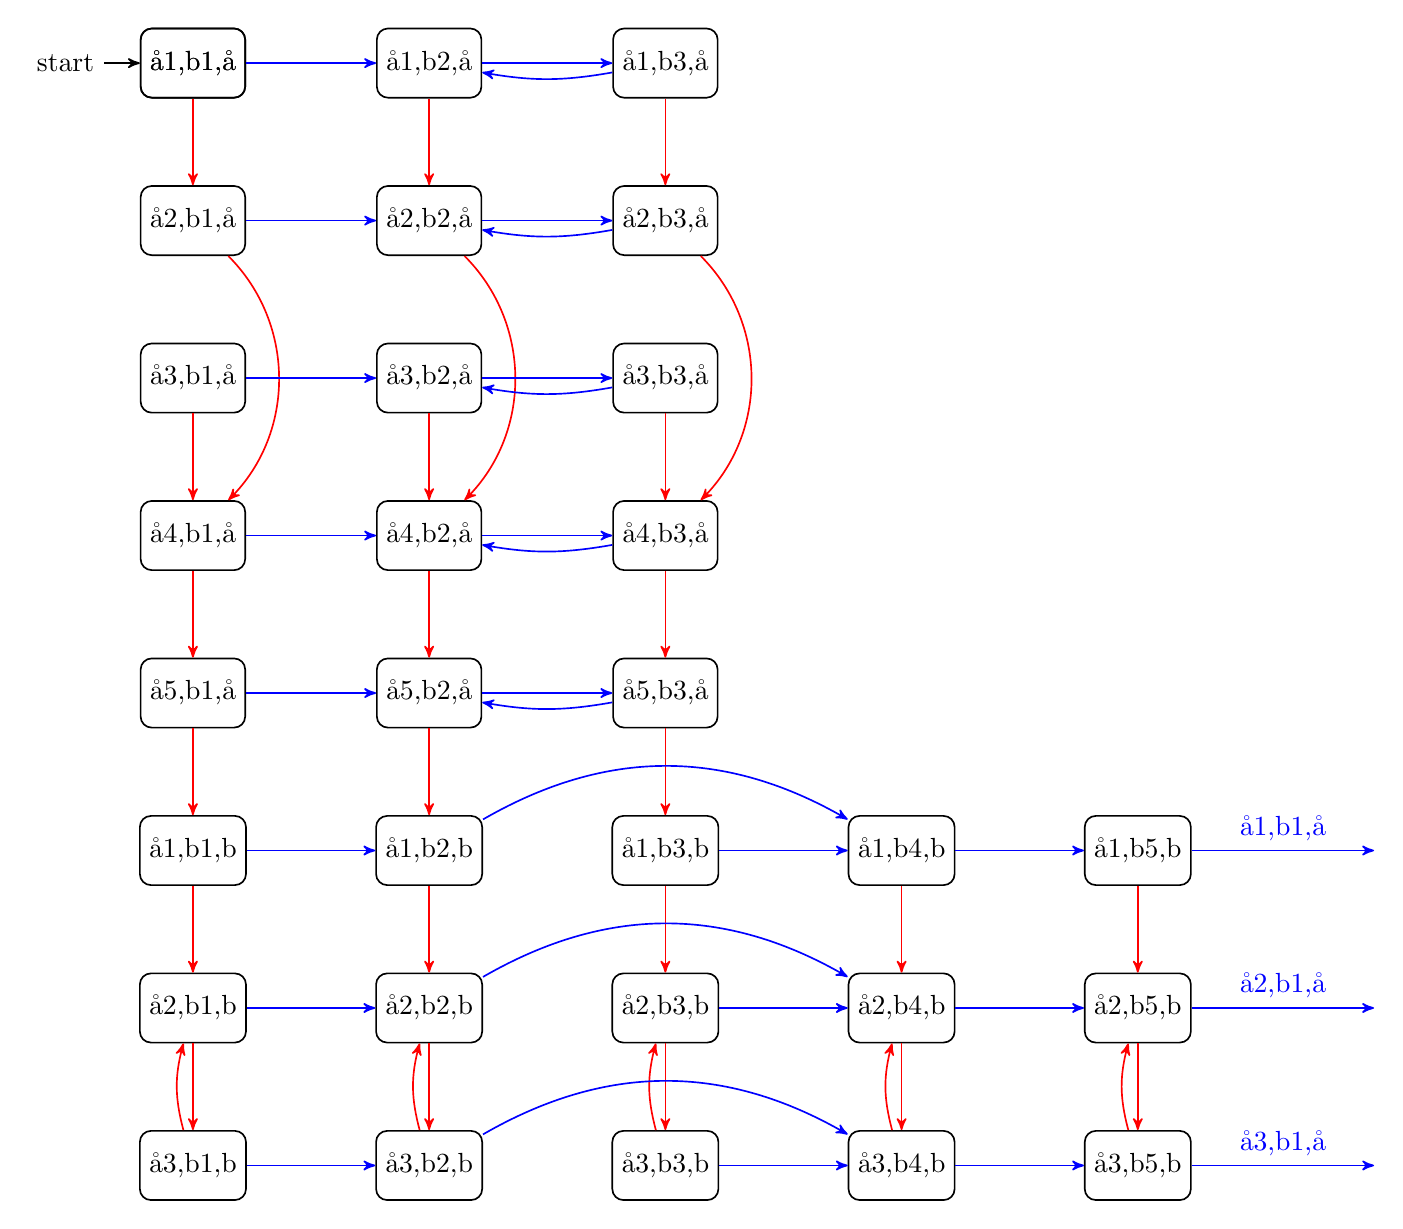
\begin{tikzpicture}[->,>=stealth',auto,node distance=2.8cm,semithick]
			\tikzset{every state/.append style={rectangle, rounded corners}}
			\node[state, initial] at (0,0) () {\r{a1},\g{b1},\r a};
			% 1: U
			% 2: while dran != a do
			% 3:	NOP
			% 4: K
			% 5: dran <- b

			% \foreach \y/\b in {0/b1,3/b2,6/b3} {
				% \foreach \x/\a in {0/a1,2/a2,4/a4,6/a5} {

			%! dran = a
			\foreach \b [count=\y from 0] in {b1,b2,b3} {
				\foreach \a [count=\x from 0] in {a1,a2,a3,a4,a5} {
					\node[state] at (\y*3,-\x*2) (\a_\b_a) {\r\a,\g\b,\r a};
				}
			}
			%! progress a
			\foreach \y in {b1,b2,b3} {
				\foreach \fromx/\tox in {a1/a2,a4/a5} {
					\draw (\fromx_\y_a) edge[red] (\tox_\y_a);
				}
				\draw (a2_\y_a) edge[red, bend left=45] (a4_\y_a);
				\draw (a3_\y_a) edge[red] (a4_\y_a);
			}
			%! progress b
			\foreach \x in {a1,a2,a3,a4,a5} {
				\foreach \fromy/\toy in {b1/b2,b2/b3} {
					\draw (\x_\fromy_a) edge[blue] (\x_\toy_a);
				}
				\draw (\x_b3_a) edge[blue,bend left=10] (\x_b2_a);
			}

			%! dran = b
			\foreach \b [count=\y from 0] in {b1,b2,b3,b4,b5} {
				\foreach \a [count=\x from 5] in {a1,a2,a3} {
					\node[state] at (\y*3,-\x*2) (\a_\b_b) {\r\a,\g\b,\g b};
				}
			}

			%! a5 => a1, dran <- b
			\foreach \y in {b1,b2,b3} {
				\draw (a5_\y_a) edge[red] (a1_\y_b);
			}

			%! progress a
			\foreach \y in {b1,b2,b3,b4,b5} {
				\foreach \fromx/\tox in {a1/a2,a2/a3} {
					\draw (\fromx_\y_b) edge[red] (\tox_\y_b);
				}
				\draw (a3_\y_b) edge[red,bend left=15] (a2_\y_b);
			}
			%! progress b
			\foreach \x in {a1,a2,a3} {
				\foreach \fromy/\toy in {b1/b2,b4/b5} {
					\draw (\x_\fromy_b) edge[blue] (\x_\toy_b);
				}
				\draw (\x_b2_b) edge[blue,bend left] (\x_b4_b);
				\draw (\x_b3_b) edge[blue] (\x_b4_b);
			}
			%! progress b, to a?_b1_a
			\foreach \a in {a1,a2,a3}
				\draw (\a_b5_b) edge[blue] node {\r\a,\g{b1},\r{a}} ++(3,0);
			% \draw (a2_b5_b) edge[blue] node {\r{a2},\g{b1},\r{a}} ++(3,0);
		\end{tikzpicture}
		\caption{Teilaufgabe a)}
	\end{figure}

\end{description}
\end{document}
